% Learning LaTeX (c) by Kerren Ortlepp

% Learning LaTeX is licensed under a
% Creative Commons Attribution-NonCommercial-ShareAlike 4.0 International License.

% You should have received a copy of the license along with this
% work. If not, see http://creativecommons.org/licenses/by-nc-sa/4.0/.
\documentclass{standalone}
\usepackage{tikz}
\usepackage{amsmath}
\usepackage{pgfplots}
\usepackage{siunitx}
\usepackage{xcolor}

\usepackage{ifthen}
\ifthenelse{\isundefined{\samplesize}}
{
    \newcommand{\samplesize}{500}
}
{
}


% Check out https://www.sharelatex.com/blog/2013/08/29/tikz-series-pt3.html for details on the flow diagram building blocks!
\definecolor{decisionColour}{HTML}{B2D1E5}
\definecolor{processColour}{HTML}{E9F2F9}
\definecolor{extraNodeColour}{HTML}{6FB7E9}
\usetikzlibrary{shapes.geometric, arrows}
\tikzstyle{start} = [circle, minimum width=0.5cm, minimum height=0.5cm,text centered, draw=black, fill=black!100, yshift=-0.3cm]
\tikzstyle{end} = [circle, minimum width=0.5cm, minimum height=0.5cm,text centered, draw=black, fill=black!0, yshift=-0.3cm, ultra thick]
\tikzstyle{process} = [rectangle, minimum width=3cm, minimum height=1cm, text centered, draw=black, fill=processColour, rounded corners=0.1cm]
\tikzstyle{decision} = [diamond, text badly centered, draw=black, fill=decisionColour, text width = 3cm]
\tikzstyle{extraNode} = [diamond, minimum width=0.25cm, minimum height=0.25cm, text centered, draw=black, fill=extraNodeColour]
\tikzstyle{arrow} = [thick,->,>=stealth]

\begin{document}%
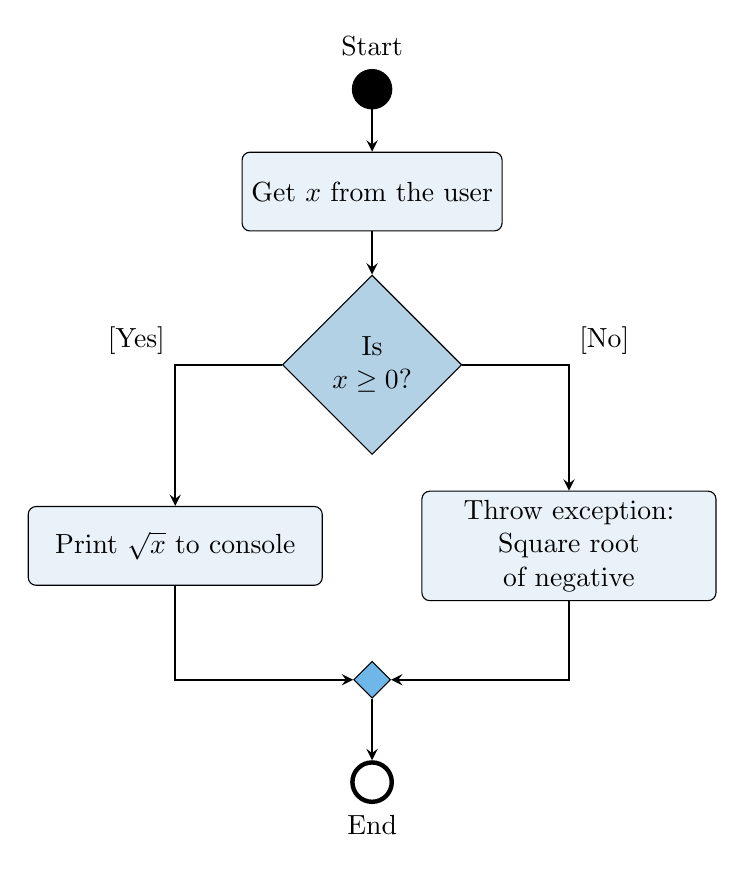
\begin{tikzpicture}
    \node (start) [start] {} node[anchor=south] {Start};

    \node (procInput) [process, below of = start, yshift=-0.3cm] {Get $x$ from the user};

    % Change the text width and minimum height to get it to look good, it's best to keep them the same so that the decision block is symmetric!
    \node (if1) [decision, below of = procInput, text width = 1.1cm, minimum height = 1.1cm, yshift=-1.2cm] {Is\\ $x \geq 0$?};

    \node (procXGreater)  [process, left of = if1, yshift=-2.3cm, xshift=-1.5cm, text width = 3.5cm] {Print $\sqrt{x}$ to console};

    \node (procXLower)  [process, right of = if1, yshift=-2.3cm, xshift=1.5cm, text width = 3.5cm] {Throw exception:\\Square root of negative};

    \node (finalNode) [extraNode, below of = if1, yshift = -3cm] {};

    \node (end) [end, below of = finalNode] {};
    \draw (end) node[anchor=north, yshift=-0.3cm] {End};

    \draw [arrow] (start) -- (procInput);
    \draw [arrow] (procInput) -- (if1);
    \draw [arrow] (if1) -| node[anchor=south east] {[Yes]} (procXGreater);
    % The -| means horizontal then vertical line
    % That means that |- would draw a vertical line first and then a horizontal. Change them around to see what they do!
    \draw [arrow] (if1) -| node[anchor=south west] {[No]} (procXLower);
    \draw [arrow] (procXGreater) |- (finalNode);
    \draw [arrow] (procXLower) |- (finalNode);
    \draw [arrow] (finalNode) -- (end);

\end{tikzpicture}
\end{document}